% Generated by code/src/report/make_figures.py from supplementary/experimental_results.
% Do not edit by hand; rerun the script instead.
\documentclass[border=6pt]{standalone}
\usepackage[T1]{fontenc}
\usepackage{helvet}
\renewcommand{\familydefault}{\sfdefault}
\usepackage{pgfplots}
\pgfplotsset{compat=1.17}
\usepgfplotslibrary{groupplots}
\definecolor{wsl}{HTML}{1F4E8C}
\definecolor{wsl2}{HTML}{7FA7D9}
\definecolor{vm}{HTML}{B35C00}
\definecolor{vm2}{HTML}{F2B66D}
\definecolor{bad}{HTML}{C0392B}
\definecolor{good}{HTML}{2E9D57}
\begin{document}
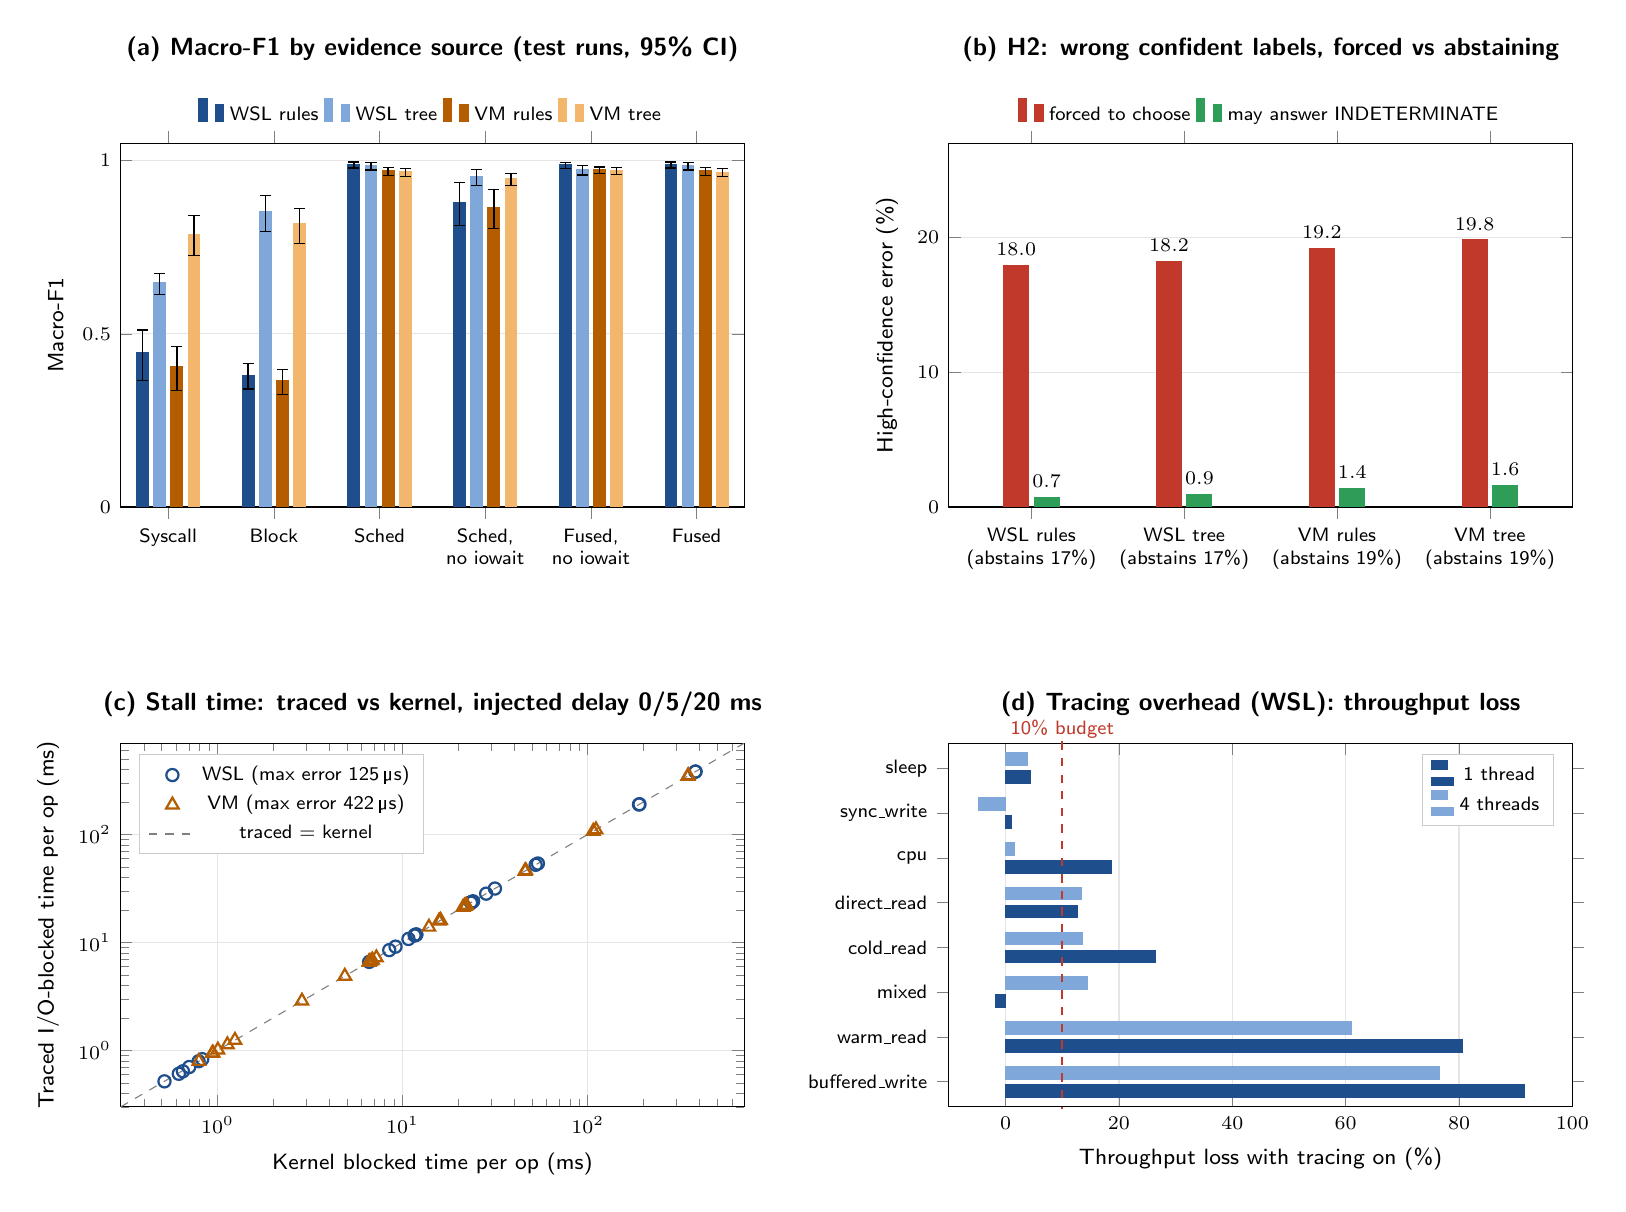
\begin{tikzpicture}[font=\footnotesize]
\begin{groupplot}[group style={group size=2 by 2, horizontal sep=26mm, vertical sep=30mm},
  width=95mm, height=62mm, title style={font=\bfseries\small, align=center},
  tick label style={font=\scriptsize}, label style={font=\footnotesize},
  legend style={font=\scriptsize, draw=none, fill=none, legend columns=4,
                at={(0.5,1.02)}, anchor=south}, ymajorgrids, grid style={gray!20}]

% (a) macro-F1 by evidence source
\nextgroupplot[title={(a) Macro-F1 by evidence source (test runs, 95\% CI)},
  title style={yshift=7mm},
  ybar, bar width=4.2pt, ymin=0, ymax=1.05, ylabel={Macro-F1},
  xtick={0,...,5}, xticklabels={{Syscall},{Block},{Sched},{Sched,\\no iowait},{Fused,\\no iowait},{Fused}}, xticklabel style={align=center},
  enlarge x limits=0.09, error bars/error bar style={line width=0.5pt, black}]
\addplot+[fill=wsl, draw=wsl, error bars/.cd, y dir=both, y explicit] coordinates {(0,0.4444) +- (0,0) += (0,0.0665) -= (0,0.0798) (1,0.3800) +- (0,0) += (0,0.0346) -= (0,0.0395) (2,0.9892) +- (0,0) += (0,0.0067) -= (0,0.0105) (3,0.8790) +- (0,0) += (0,0.0581) -= (0,0.0663) (4,0.9884) +- (0,0) += (0,0.0068) -= (0,0.0101) (5,0.9892) +- (0,0) += (0,0.0067) -= (0,0.0105)};
\addplot+[fill=wsl2, draw=wsl2, error bars/.cd, y dir=both, y explicit] coordinates {(0,0.6465) +- (0,0) += (0,0.0267) -= (0,0.0341) (1,0.8519) +- (0,0) += (0,0.0463) -= (0,0.0574) (2,0.9857) +- (0,0) += (0,0.0087) -= (0,0.0127) (3,0.9546) +- (0,0) += (0,0.0206) -= (0,0.0277) (4,0.9741) +- (0,0) += (0,0.0115) -= (0,0.0157) (5,0.9857) +- (0,0) += (0,0.0087) -= (0,0.0127)};
\addplot+[fill=vm, draw=vm, error bars/.cd, y dir=both, y explicit] coordinates {(0,0.4047) +- (0,0) += (0,0.0585) -= (0,0.0677) (1,0.3636) +- (0,0) += (0,0.0336) -= (0,0.0400) (2,0.9706) +- (0,0) += (0,0.0093) -= (0,0.0124) (3,0.8632) +- (0,0) += (0,0.0531) -= (0,0.0584) (4,0.9744) +- (0,0) += (0,0.0071) -= (0,0.0106) (5,0.9706) +- (0,0) += (0,0.0093) -= (0,0.0124)};
\addplot+[fill=vm2, draw=vm2, error bars/.cd, y dir=both, y explicit] coordinates {(0,0.7878) +- (0,0) += (0,0.0530) -= (0,0.0630) (1,0.8184) +- (0,0) += (0,0.0422) -= (0,0.0588) (2,0.9686) +- (0,0) += (0,0.0098) -= (0,0.0132) (3,0.9473) +- (0,0) += (0,0.0148) -= (0,0.0192) (4,0.9713) +- (0,0) += (0,0.0076) -= (0,0.0112) (5,0.9664) +- (0,0) += (0,0.0097) -= (0,0.0129)};
\legend{WSL rules, WSL tree, VM rules, VM tree}

% (b) H2: abstention
\nextgroupplot[title={(b) H2: wrong confident labels, forced vs abstaining},
  title style={yshift=7mm},
  ybar, bar width=9pt, ymin=0, ymax=27, ylabel={High-confidence error (\%)},
  xtick={0,...,3}, xticklabels={{WSL rules\\(abstains 17\%)},{WSL tree\\(abstains 17\%)},{VM rules\\(abstains 19\%)},{VM tree\\(abstains 19\%)}}, xticklabel style={align=center},
  enlarge x limits=0.18, nodes near coords, nodes near coords style={font=\scriptsize, text=black},
  every node near coord/.append style={/pgf/number format/.cd, fixed, fixed zerofill, precision=1}]
\addplot+[fill=bad, draw=bad] coordinates {(0,17.96) (1,18.21) (2,19.19) (3,19.83)};
\addplot+[fill=good, draw=good] coordinates {(0,0.71) (1,0.91) (2,1.37) (3,1.60)};
\legend{forced to choose, may answer INDETERMINATE}

% (c) delay sweep
\nextgroupplot[title={(c) Stall time: traced vs kernel, injected delay 0/5/20 ms},
  xmode=log, ymode=log, xmin=0.3, xmax=700, ymin=0.3, ymax=700,
  xlabel={Kernel blocked time per op (ms)}, ylabel={Traced I/O-blocked time per op (ms)},
  xmajorgrids, legend style={at={(0.03,0.97)}, anchor=north west, legend columns=1,
  fill=white, draw=gray!40}]
\addplot[only marks, mark=o, mark size=2.2pt, wsl, thick] coordinates {(0.7036,0.7011) (11.6901,11.6934) (23.5604,23.5626) (0.7911,0.7933) (11.6812,11.6862) (23.6420,23.6463) (0.6505,0.6405) (11.7313,11.7269) (23.7007,23.6979) (0.8277,0.8291) (11.8622,11.8655) (24.0302,24.0286) (0.5173,0.5167) (11.8401,11.7650) (23.6305,23.6016) (0.6183,0.6070) (11.6087,11.6083) (23.4034,23.3493) (9.1563,9.1350) (189.1268,189.1828) (381.2031,381.2610) (8.4715,8.4841) (190.4265,190.4869) (382.4618,382.4952) (6.5983,6.6018) (28.2754,28.2811) (52.3076,52.3134) (10.7530,10.7612) (31.5292,31.5322) (53.8131,53.8189)};
\addplot[only marks, mark=triangle, mark size=2.6pt, vm, thick] coordinates {(0.9456,0.9481) (6.6566,6.6660) (21.6813,21.6862) (1.2424,1.2442) (6.8711,6.8804) (21.2355,21.2410) (0.9382,0.9421) (6.6004,6.6039) (22.1471,22.1478) (1.0048,1.0114) (7.2173,7.2188) (21.8705,21.8701) (1.1314,1.1311) (6.5788,6.5833) (21.5883,21.5866) (0.7930,0.7928) (6.7996,6.7626) (21.6139,21.6014) (13.8697,13.8778) (107.1876,107.2740) (347.1630,347.2903) (15.9550,15.9612) (110.7340,110.8101) (350.3141,350.3699) (2.8594,2.8695) (15.7264,15.7789) (45.7589,45.7971) (4.8739,4.8761) (16.0317,16.0371) (46.3021,46.3051)};
\addplot[gray, dashed, domain=0.3:700, samples=2] {x};
\legend{WSL (max error 125\,\textmu s), VM (max error 422\,\textmu s), traced = kernel}

% (d) overhead
\nextgroupplot[title={(d) Tracing overhead (WSL): throughput loss},
  xbar, bar width=4.5pt, xmin=-10, xmax=100, xlabel={Throughput loss with tracing on (\%)},
  ytick={0,...,7}, yticklabels={{sleep},{sync\_write},{cpu},{direct\_read},{cold\_read},{mixed},{warm\_read},{buffered\_write}}, y dir=reverse,
  enlarge y limits=0.08, ymajorgrids=false, xmajorgrids, clip=false,
  legend style={at={(0.97,0.97)}, anchor=north east, legend columns=1, fill=white, draw=gray!40}]
\addplot+[fill=wsl, draw=wsl] coordinates {(4.3,0) (1.1,1) (18.7,2) (12.6,3) (26.5,4) (-1.8,5) (80.6,6) (91.5,7)};
\addplot+[fill=wsl2, draw=wsl2] coordinates {(3.8,0) (-4.7,1) (1.5,2) (13.3,3) (13.6,4) (14.5,5) (61.1,6) (76.5,7)};
\draw[bad, thick, dashed] (axis cs:10,-0.6) -- (axis cs:10,7.6);
\node[bad, font=\scriptsize, anchor=south, fill=white, inner sep=1pt] at (axis cs:10,-0.6) {10\% budget};
\legend{1 thread, 4 threads}
\end{groupplot}
\end{tikzpicture}
\end{document}
